%%
%% This is file `sample-sigconf.tex',
%% generated with the docstrip utility.
%%
%% The original source files were:
%%
%% samples.dtx  (with options: `all,proceedings,bibtex,sigconf')
%% 
%% IMPORTANT NOTICE:
%% 
%% For the copyright see the source file.
%% 
%% Any modified versions of this file must be renamed
%% with new filenames distinct from sample-sigconf.tex.
%% 
%% For distribution of the original source see the terms
%% for copying and modification in the file samples.dtx.
%% 
%% This generated file may be distributed as long as the
%% original source files, as listed above, are part of the
%% same distribution. (The sources need not necessarily be
%% in the same archive or directory.)
%%
%%
%% Commands for TeXCount
%TC:macro \cite [option:text,text]
%TC:macro \citep [option:text,text]
%TC:macro \citet [option:text,text]
%TC:envir table 0 1
%TC:envir table* 0 1
%TC:envir tabular [ignore] word
%TC:envir displaymath 0 word
%TC:envir math 0 word
%TC:envir comment 0 0
%%
%% The first command in your LaTeX source must be the \documentclass
%% command.
%%
%% For submission and review of your manuscript please change the
%% command to \documentclass[manuscript, screen, review]{acmart}.
%%
%% When submitting camera ready or to TAPS, please change the command
%% to \documentclass[sigconf]{acmart} or whichever template is required
%% for your publication.
%%
%%
\documentclass[sigconf,nonacm,review,language=english,language=german]{acmart}
%%
%% \BibTeX command to typeset BibTeX logo in the docs
\AtBeginDocument{%
  \providecommand\BibTeX{{%
    Bib\TeX}}}

\usepackage[german,english]{babel}

% Caption Packet
\usepackage[margin=0pt,font=small,labelfont=bf]{caption}
\usepackage{subcaption}

% Algorithmen
\usepackage[section]{algorithm}
\usepackage{algorithmic}

% TikZ
\usepackage{tikz}
\usetikzlibrary{positioning}
\usetikzlibrary{calc}
\usetikzlibrary{automata}

% Links
\usepackage{hyperref}
\hypersetup{
  colorlinks   = true, % Colours links instead of ugly boxes
  urlcolor     = blue, % Colour for external hyperlinks
  linkcolor    = blue, % Colour of internal links
  citecolor   = red % Colour of citations
}

%% Rights management information.  This information is sent to you
%% when you complete the rights form.  These commands have SAMPLE
%% values in them; it is your responsibility as an author to replace
%% the commands and values with those provided to you when you
%% complete the rights form.
\setcopyright{acmlicensed}
\copyrightyear{2018}
\acmYear{2018}
\acmDOI{XXXXXXX.XXXXXXX}
%% These commands are for a PROCEEDINGS abstract or paper.
\acmConference[Conference acronym 'XX]{Make sure to enter the correct
  conference title from your rights confirmation email}{June 03--05,
  2018}{Woodstock, NY}
%%
%%  Uncomment \acmBooktitle if the title of the proceedings is different
%%  from ``Proceedings of ...''!
%%
%%\acmBooktitle{Woodstock '18: ACM Symposium on Neural Gaze Detection,
%%  June 03--05, 2018, Woodstock, NY}
\acmISBN{978-1-4503-XXXX-X/2018/06}


%%
%% Submission ID.
%% Use this when submitting an article to a sponsored event. You'll
%% receive a unique submission ID from the organizers
%% of the event, and this ID should be used as the parameter to this command.
%%\acmSubmissionID{123-A56-BU3}

%%
%% For managing citations, it is recommended to use bibliography
%% files in BibTeX format.
%%
%% You can then either use BibTeX with the ACM-Reference-Format style,
%% or BibLaTeX with the acmnumeric or acmauthoryear sytles, that include
%% support for advanced citation of software artefact from the
%% biblatex-software package, also separately available on CTAN.
%%
%% Look at the sample-*-biblatex.tex files for templates showcasing
%% the biblatex styles.
%%

%%
%% The majority of ACM publications use numbered citations and
%% references.  The command \citestyle{authoryear} switches to the
%% "author year" style.
%%
%% If you are preparing content for an event
%% sponsored by ACM SIGGRAPH, you must use the "author year" style of
%% citations and references.
%% Uncommenting
%% the next command will enable that style.
%%\citestyle{acmauthoryear}


%%
%% end of the preamble, start of the body of the document source.
\begin{document}

%%
%% The "title" command has an optional parameter,
%% allowing the author to define a "short title" to be used in page headers.
\title{Routingalgorithmen Report}

%%
%% The "author" command and its associated commands are used to define
%% the authors and their affiliations.
%% Of note is the shared affiliation of the first two authors, and the
%% "authornote" and "authornotemark" commands
%% used to denote shared contribution to the research.
\author{Yannik Buchner}
\affiliation{%
  \institution{TU Dortmund}
  \city{Dortmund}
  \country{Germany}
}
\email{yannic.buchner@tu-dortmund.de}

\author{Simon Buschmann}
\affiliation{%
  \institution{TU Dortmund}
  \city{Dortmund}
  \country{Germany}
}
\email{simon-thomas.buschmann@tu-dortmund.de}

\author{Jan Draeger}
\affiliation{%
  \institution{TU Dortmund}
  \city{Dortmund}
  \country{Germany}
}
\email{jan.draeger@tu-dortmund.de}

\author{Nikita Podibko}
\affiliation{%
  \institution{TU Dortmund}
  \city{Dortmund}
  \country{Germany}
}
\email{nikita.podibko@tu-dortmund.de}

\author{Johannes Heinrich}
\affiliation{%
  \institution{TU Dortmund}
  \city{Dortmund}
  \country{Germany}
}
\email{johannes.heinrich@tu-dortmund.de}

\author{Malek Haoues Rhaiem}
\affiliation{%
  \institution{TU Dortmund}
  \city{Dortmund}
  \country{Germany}
}
\email{malek.haoues-rhaiem@tu-dortmund.de}



%%
%% By default, the full list of authors will be used in the page
%% headers. Often, this list is too long, and will overlap
%% other information printed in the page headers. This command allows
%% the author to define a more concise list
%% of authors' names for this purpose.
\renewcommand{\shortauthors}{Buchner et al.}

%%
%% The abstract is a short summary of the work to be presented in the
%% article.
\begin{abstract}
Eine gängige Praxis im Traffic Engineering ist es, die Gewichte der Links im Netzwerk zu optimieren, um dann den Traffic auf den kürzesten Pfaden anhand von ECMP zu routen. Diese Herangehensweise nennt sich Link Weight Optimization (LWO) und bietet die Routing-Grundlage für einen Großteil der Internet Service Provider (ISP). Eine andere Herangehensweise ist es, Demands einzeln zu betrachten und anhand von spezifischen Kriterien sog. Wegpunkte zu setzen. Im Laufe unserer Arbeit haben wir uns mit verschiedenen Möglichkeiten beschäftigt, Waypoint Optimization (WPO) zu realisieren und auf Basis der Arbeit \textit{Traffic engineering with joint link weight and segment optimization} \cite{parham2021traffic} Möglichkeiten herausgearbeitet, WPO und LWO zu kombinieren. Außerdem beschäftigen wir uns mit einem neuen Aspekt, dem priorisierten Routing, und stellen dazu konkrete Algorithmen vor, die im Hinblick verschiedenster Kriterien in ausgiebigen Experimenten analysiert werden.
\end{abstract}

%%
%% The code below is generated by the tool at http://dl.acm.org/ccs.cfm.
%% Please copy and paste the code instead of the example below.
%%
\begin{CCSXML}
<ccs2012>
<concept>
<concept_id>10003033.10003068.10003073.10003076</concept_id>
<concept_desc>Networks~Traffic engineering algorithms</concept_desc>
<concept_significance>500</concept_significance>
</concept>
</ccs2012>
\end{CCSXML}

\ccsdesc[500]{Networks~Traffic engineering algorithms}

%%
%% Keywords. The author(s) should pick words that accurately describe
%% the work being presented. Separate the keywords with commas.
\keywords{traffic engineering, network algorithms, segment routing, priority demands}

%% A "teaser" image appears between the author and affiliation
%% information and the body of the document, and typically spans the
%% page.
\begin{teaserfigure}
  
\includegraphics[width=\textwidth]{Grafiken/netzwerk.jpeg}
  % \caption{}
  \Description{Pretty.}
  \label{fig:network}
\end{teaserfigure}

%%
%% This command processes the author and affiliation and title
%% information and builds the first part of the formatted document.
\maketitle

\section{Einleitung}
    In dieser Arbeit haben wir uns das Paper \cite{parham2021traffic} und die zwei dazugehörigen Repositories \cite{original_p1} und \cite{original_p2} angeschaut. Dabei haben wir versucht, die Ergebnisse zu reproduzieren. Auch haben wir uns drei weitere Algorithmen überlegt und diese in das bestehende Projekt eingearbeitet. Unsere Erweiterungen kann man hier finden \cite{reproduktion_p1} und \cite{reproduktion_p2}.
    Innerhalb dieses Reportes stellen wir unsere Ergebnisse bei der Einarbeitung unserer eigenen drei Algorithmen vor. Wir erläutern dabei die Idee der Algorithmen, die jeweiligen Vor- und Nachteile, die Schwierigkeiten, welche wir bei der Einarbeitung in die beiden Projekte hatten, und die Ergebnisse, die wir mit den Algorithmen erzielt haben. Zum Schluss gehen wir noch auf die Reproduktion der Gruppe 4 ein, welche auch zwei eigene Algorithmen entwickelt hat. 


\section{Projekt 1}
Im folgenden Teil werden die Vorgehensweise und die Ergebnisse des ersten Projekts vorgestellt. Dabei stand die Frage im Fokus, wie sich verschiedene Zielfunktionen mithilfe geeigneter Algorithmen möglichst optimal erfüllen lassen
    \subsection{Algorithmen}
        Die drei Algorithmen, die wir erstellt haben, sind Least Loaded Link First (LLLF), Randomized Load Aware Path Selection (RLAPS) und Apl Waypoints. 
        
        \paragraph{3.1.1   LLLF}
            Der \textit{Least Loaded Link First} (LLLF) Algorithmus ist ein heuristisches Verfahren zur Pfadwahl in Kommunikationsnetzen. Ziel ist es, Anfragen für Datenübertragungen so durch das Netzwerk zu leiten, dass die Auslastung einzelner Kanten möglichst gleichmäßig verteilt wird (Maximum Link Utilisation MLU). \\
            Der LLLF-Algorithmus betrachtet die aktuelle Belastung der Netzwerkressourcen. Für jeden Demand wird ein Pfad gesucht, der die aktuelle maximale Auslastung des Netzes minimal hält. Dies geschieht durch eine Abwandlung des Dijkstra-Algorithmus, der die relative Auslastung der Links betrachtet.
            \begin{itemize}
                \item Fairness: Es wird vermieden, wiederholt denselben, zu verwenden.
                \item Greedy-Heuristik: Es wird eine lokal optimale Entscheidung für die aktuelle Anfrage, ohne globale Optimierung über alle Demands hinweg, getroffen.
                \item Laufzeit: Der Algorithmus läuft effizient, wobei die Laufzeit ungefähr der von Dijkstra entspricht.
                \item Praktische Relevanz: In großen Telekommunikations- und Datennetzen ist LLLF attraktiv, weil er relativ einfach implementierbar ist.
            \end{itemize}
            
                
         \paragraph{3.1.2   RLAPS}
            Der Algorithmus Randomized Load-Aware Path Selection (RLAPS) ist ein heuristisches Routingverfahren, das entwickelt wurde, um Netzwerke gegen lokale Überlastung abzusichern und dabei dennoch kurze Pfade zu berücksichtigen. Anstelle deterministischer Shortest-Path-Strategien, die häufig zur Ausbildung von Hotspots führen, nutzt der Ansatz kontrollierte Randomisierung, um Diversität in der Pfadwahl zu erzeugen und dadurch den Datenverkehr gleichmäßiger im Netz zu verteilen. 
            Die Grundidee besteht darin, für jeden Demand aus eine Menge von k-kürzesten Pfaden drei Kandidaten zufällig zu wählen und mit einer lastbasierten Bewertungsfunktion den besten zu wählen. Sei $P$ ein Pfad bestehend aus Kanten $(e_1,\dots,e_m)$ und $d$ die Demand-Größe. Mit $f_e$ der bisher auf $e$ geplanten Last und $c_e$ der Kapazität gilt die Pfadbewertungsfunktion
            $$
            \mathrm{score}(P,d) \,=\, \sum_{e\in P} \frac{f_e + d}{c_e}
            $$
            Diese Wahl zielt direkt darauf ab, die entstehende Auslastung auf den von $P$ genutzten Links zu minimieren. 
            
        \paragraph{3.1.3 \, AplWaypoints}
Der \textit{AplWaypoints}-Ansatz setzt gezielt Waypoints, um zwischen durchschnittlicher Pfadlänge (APL) und maximaler Linkauslastung (MLU) auszubalancieren. Optimiert wird die kombinierte Zielfunktion
\[
J(\lambda)=\lambda\cdot \text{APL} + (1-\lambda)\cdot \text{MLU}, \quad \lambda\in[0,1],
\]
wobei APL die nach Demand gewichtete Hop-Distanz und MLU die maximale Auslastung (Flow/Kapazität) eines Links ist. Kleine $\lambda$ priorisieren Robustheit/MLU, große $\lambda$ kurze Pfade/Latenz.

\begin{itemize}
  \item \textbf{Kandidatenwahl:} Top-$k$ Knoten mit
  \(
  k=\max\!\bigl(10,\lfloor 0.2|V|\rfloor\bigr)
  \)
  nach Score
  \(
  \mathrm{Score}(v)=\alpha\,BC(v)+\beta\,Deg(v)+\theta\,DV(v)
\),
mit Betweenness $BC$, Grad $Deg$ und Demand-Volumen $DV$ (Summe der an $v$ anliegenden Demands)
und mit Gewichten $\alpha=0{,}5$, $\beta=0{,}3$, $\theta=0{,}15$ \;(\(\alpha+\beta+\theta=1\)).

  \item \textbf{Vorberechnung:} BFS speichert Distanzen und Pfade für $(s,t)$, $(s,v)$, $(v,t)$ (gerichteter, ungewichteter Graph).
  \item \textbf{Bewertung/Update:} Für jeden Demand $(s,t,d)$ (absteigend nach $d$) werden Kandidaten $v\neq s,t$ getestet. Neuer Pfad $s\!\to\!v\!\to\!t$; Flüsse werden entlang alter/ neuer Pfade ab- bzw.\ zugerechnet, MLU neu bestimmt. APL wird per
  \[
  \Delta\text{APL}=\frac{\bigl(\text{dist}(s,v)+\text{dist}(v,t)-\text{dist}(s,t)\bigr)\cdot d}{\sum_i d_i}
  \]
  in $O(1)$ aktualisiert. Gewählt wird die Option mit minimalem $J(\lambda)$, sonst bleibt $s\!\to\!t$ direkt.
\end{itemize}

    
    
    \subsection{Experimente}
        \paragraph{3.2.1   LLLF}
            Im Rahmen der Experimente wurde der LLLF-Algorithmus, wie oben beschrieben, in das Projekt integriert. Auch wurden noch weiter kleine Verbesserungen an dem Algorithmus vorgenommen, wie die Demands zu sortieren oder die Verteilung der Demands mehrmals hintereinander durchzuführen. Da der LLLF-Algorithmus, wie die schon existierenden Algorithmen, die MLU optimiert, gab es bei dem Vergleich mit den anderen Algorithmen keinen weiten Aufwand.

        \paragraph{3.2.2   RLAPS}
            Im Rahmen der Experimente wurde der Algorithmus Randomized Load-Aware Path Selection (RLAPS) in die bestehende Testumgebung integriert. Die Implementierung selbst erwies sich vergleichsweise unkompliziert, da der Algorithmus im Kern nur auf der Berechnung von k-kürzesten Pfaden sowie einer einfachen Bewertungsfunktion basiert.
            Das Ziel der Experimente bestand nicht allein darin, die maximale Linkauslastung (MLU) zu reduzieren, sondern auch die durchschnittliche Linkauslastung (ALU) zu verbessern. Durch die randomisierte Auswahl und die lastbewusste Pfadbewertung sollte der Algorithmus eine gleichmäßigere Lastverteilung im Netzwerk ermöglichen.

        \paragraph{3.2.3   AplWaypoints}
            Als Darstellung der Fähigkeiten des APL-Waypoints Algorithmus sowie dem allgemeinen Vergleich wurden die Algorithmen LLLF, RLAPS, InverseCapacity und GreedyWaypoints im Rahmen von Experiment 1 herangezogen. Dafür wurden alle relevanten Algorithmen sowie eine Vielzahl an unterschiedlichen und bekannten Topologien innerhalb einer Testumgebung implementiert. Zum Vergleich der Algorithmen wurden die Metriken der Laufzeit, der MLU-Auslastung, der ALU-Auslastung und der APL betrachtet. In den Abbildungen \ref{fig:ergebnisse_projekt_1} werden jeweils für jede Topologie die Gruppe an Algorithmen unter Betrachtung einer ausgewählten Metrik dargestellt. Zur Darstellung wird ein Boxplot für jeden Algorithmus verwendet.
 
    \subsection{Resultate}
        Alle Algorithmen konnten gut in dem Projekt umgesetzt werden und haben sich gut in die schon vorhandenen Algorithmen integriert. In Abbildung \ref{fig:ergebnisse_projekt_1} sind die Ergebnisse der Algorithmen. Dabei haben alle Algorithmen durchschnittlich gut bei der MLU abgeschnitten, wobei bei einigen Topologien die einen Algorithmen besser waren und bei anderen Topologien die anderen Algorithmen. 

        \begin{figure*}[h]
           \centering
            \begin{subfigure}{0.49\textwidth}
                \centering
               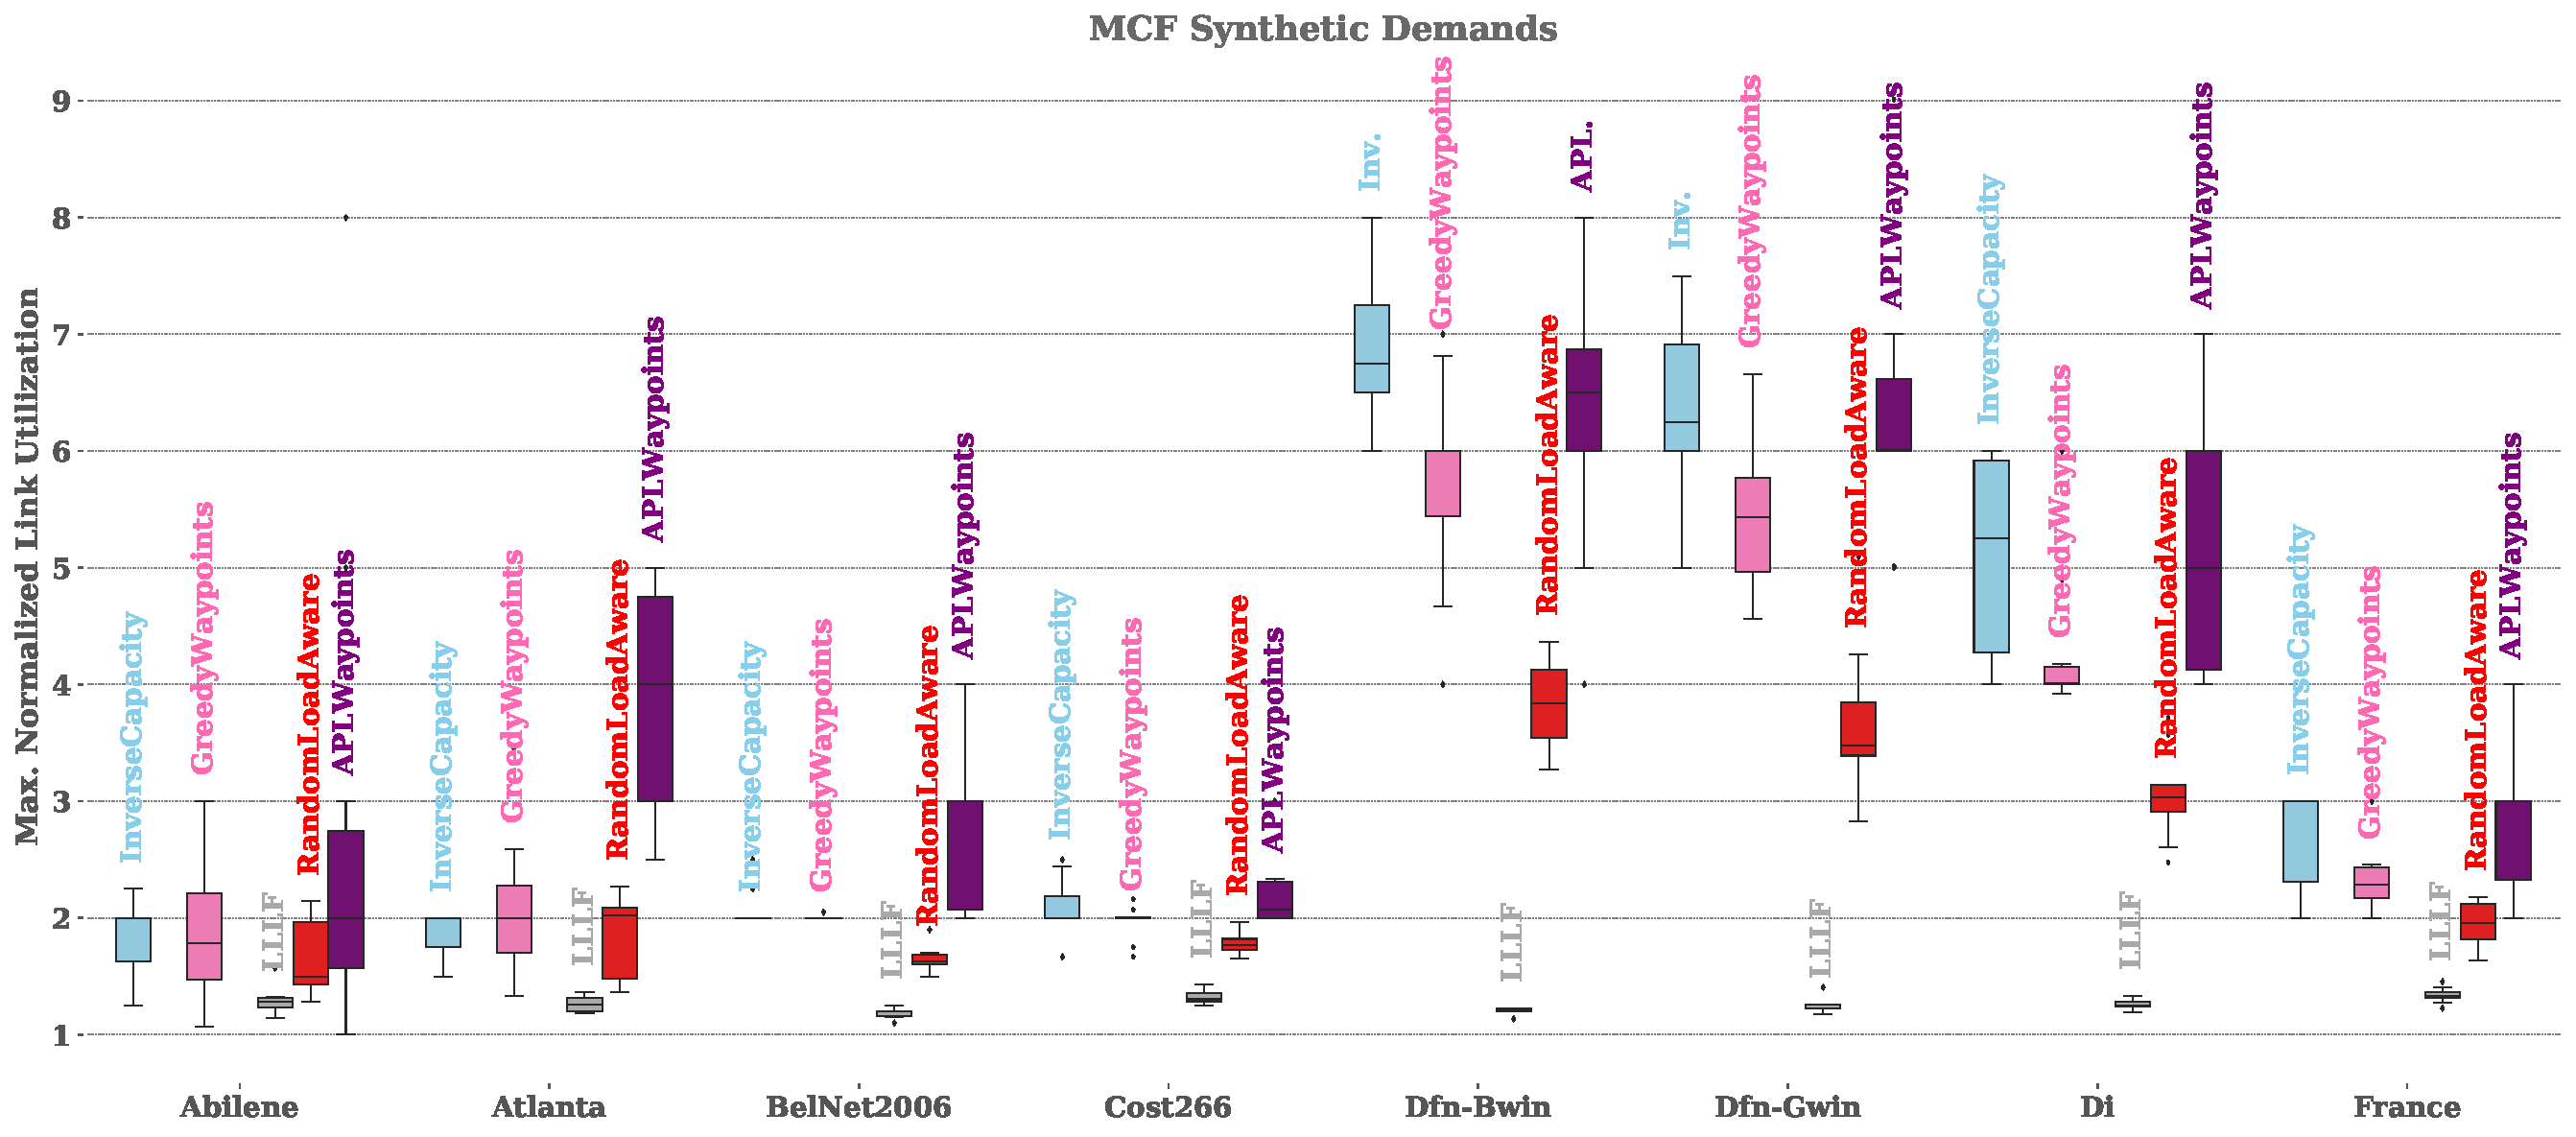
\includegraphics[width=1\linewidth]{Grafiken/all_topologies_objective_mlu_0.pdf}
               \caption{Synthetische Topologien MLU}
               \label{fig:ergebnisse_projekt_1_synt_topo_mlu}
            \end{subfigure}
            \begin{subfigure}{0.49\textwidth}
                \centering
               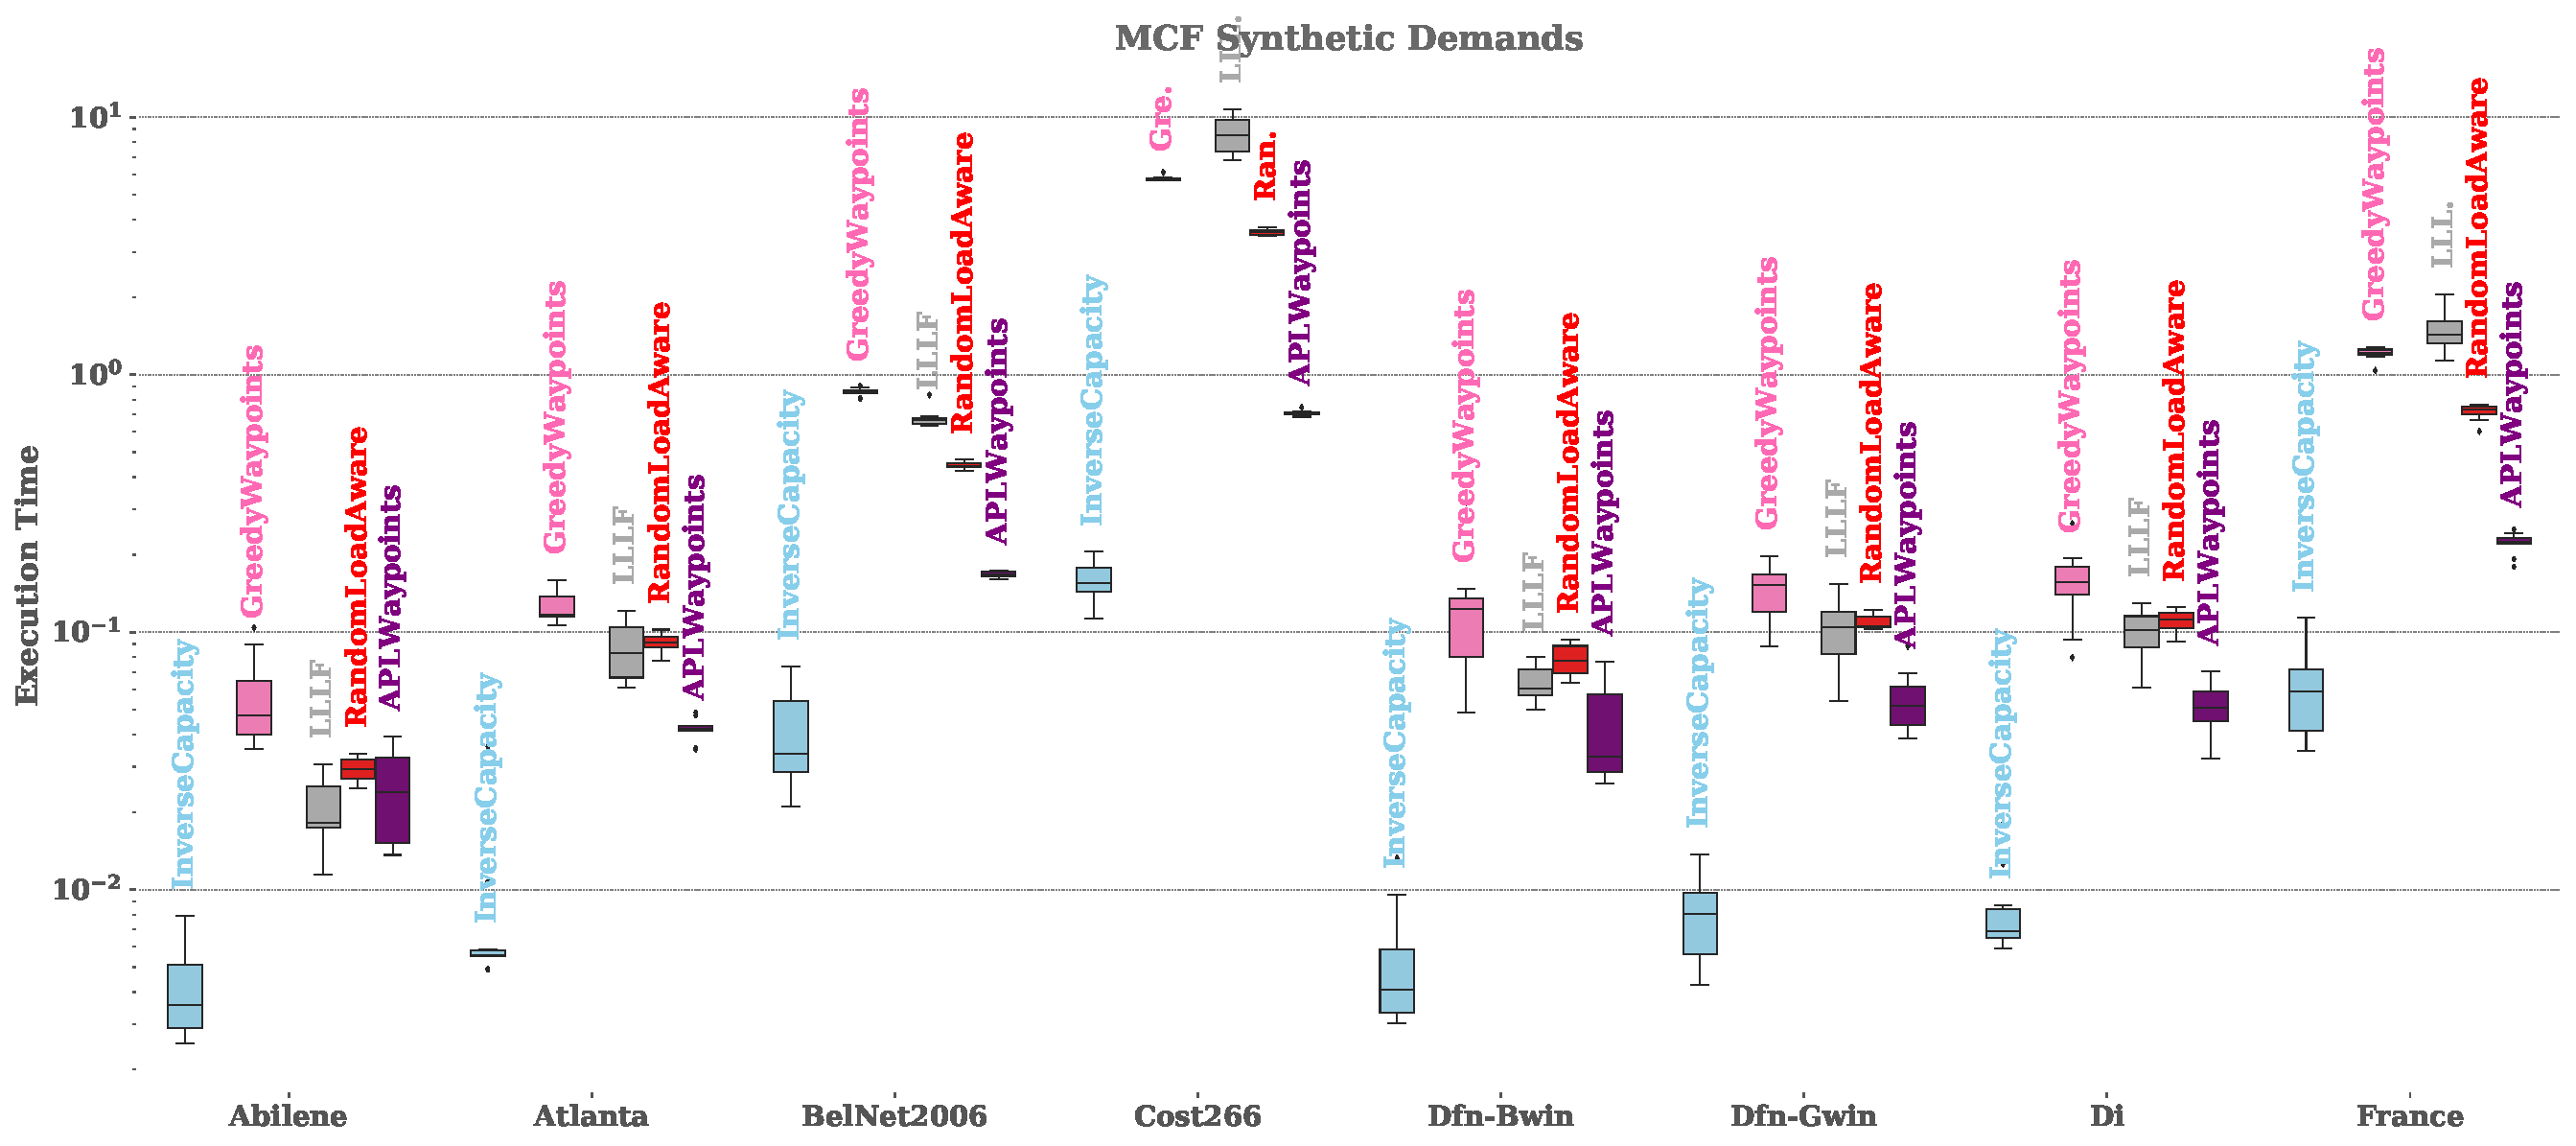
\includegraphics[width=1\linewidth]{Grafiken/projekt1/all_topologies_execution_time_0.pdf}
               \caption{Synthetische Topologien Ausführungszeit}
               \label{fig:ergebnisse_projekt_1_synt_topo_time}
            \end{subfigure}
           \begin{subfigure}{0.49\textwidth}
                \centering
               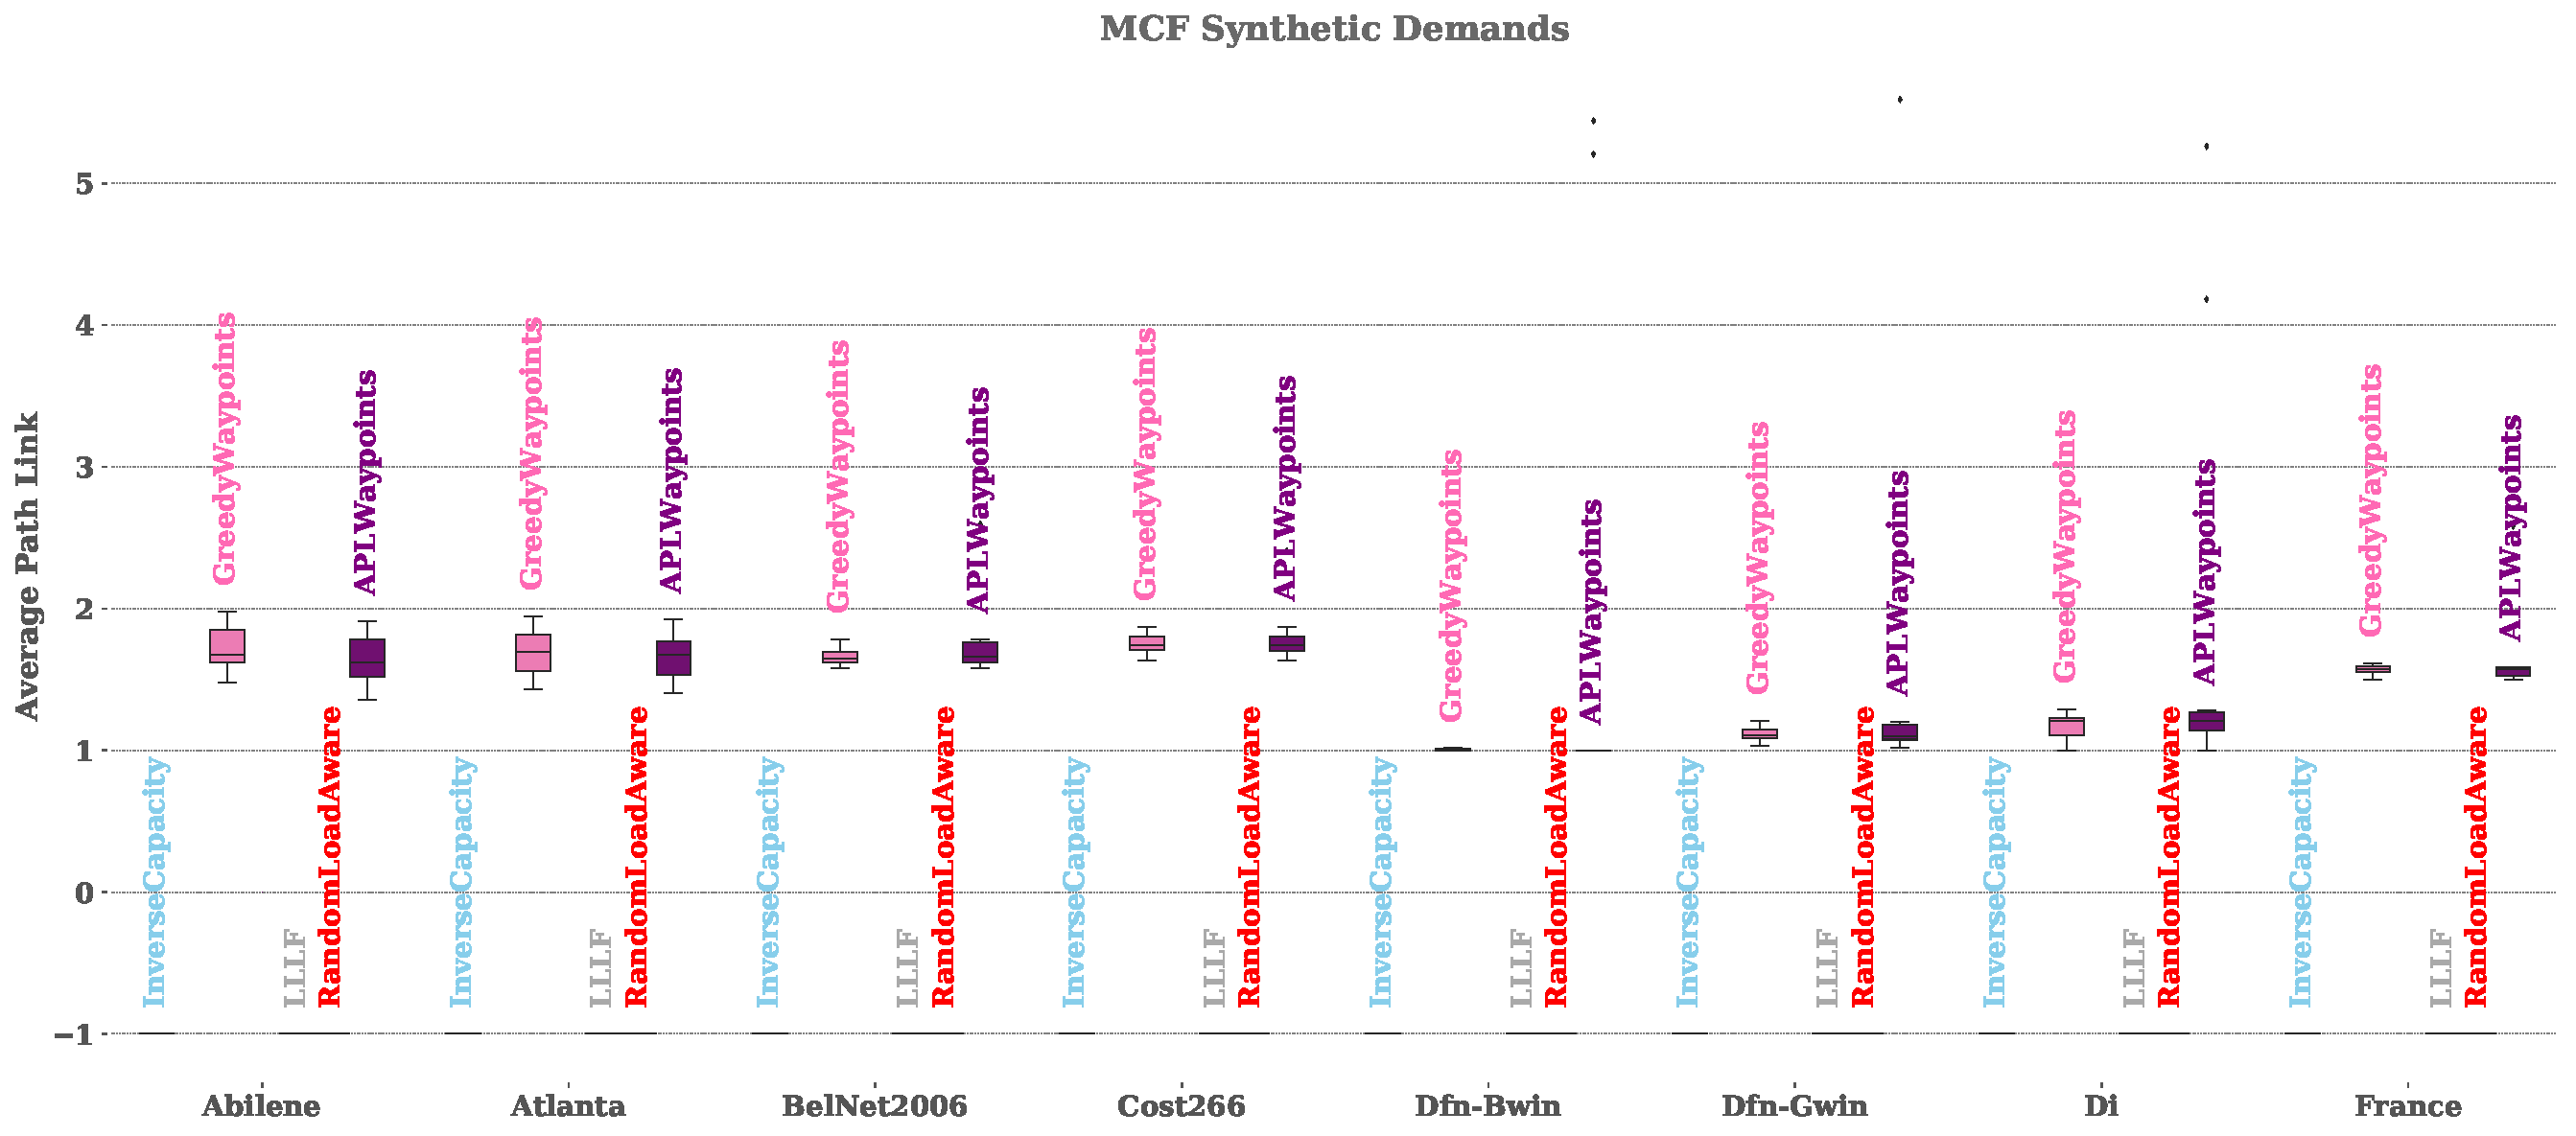
\includegraphics[width=1\linewidth]{Grafiken/projekt1/all_topologies_objective_apl_0.pdf}
               \caption{Synthetische Topologien APL}
               \label{fig:ergebnisse_projekt_1_synt_topo_apl}
            \end{subfigure}
            \begin{subfigure}{0.49\textwidth}
                \centering
               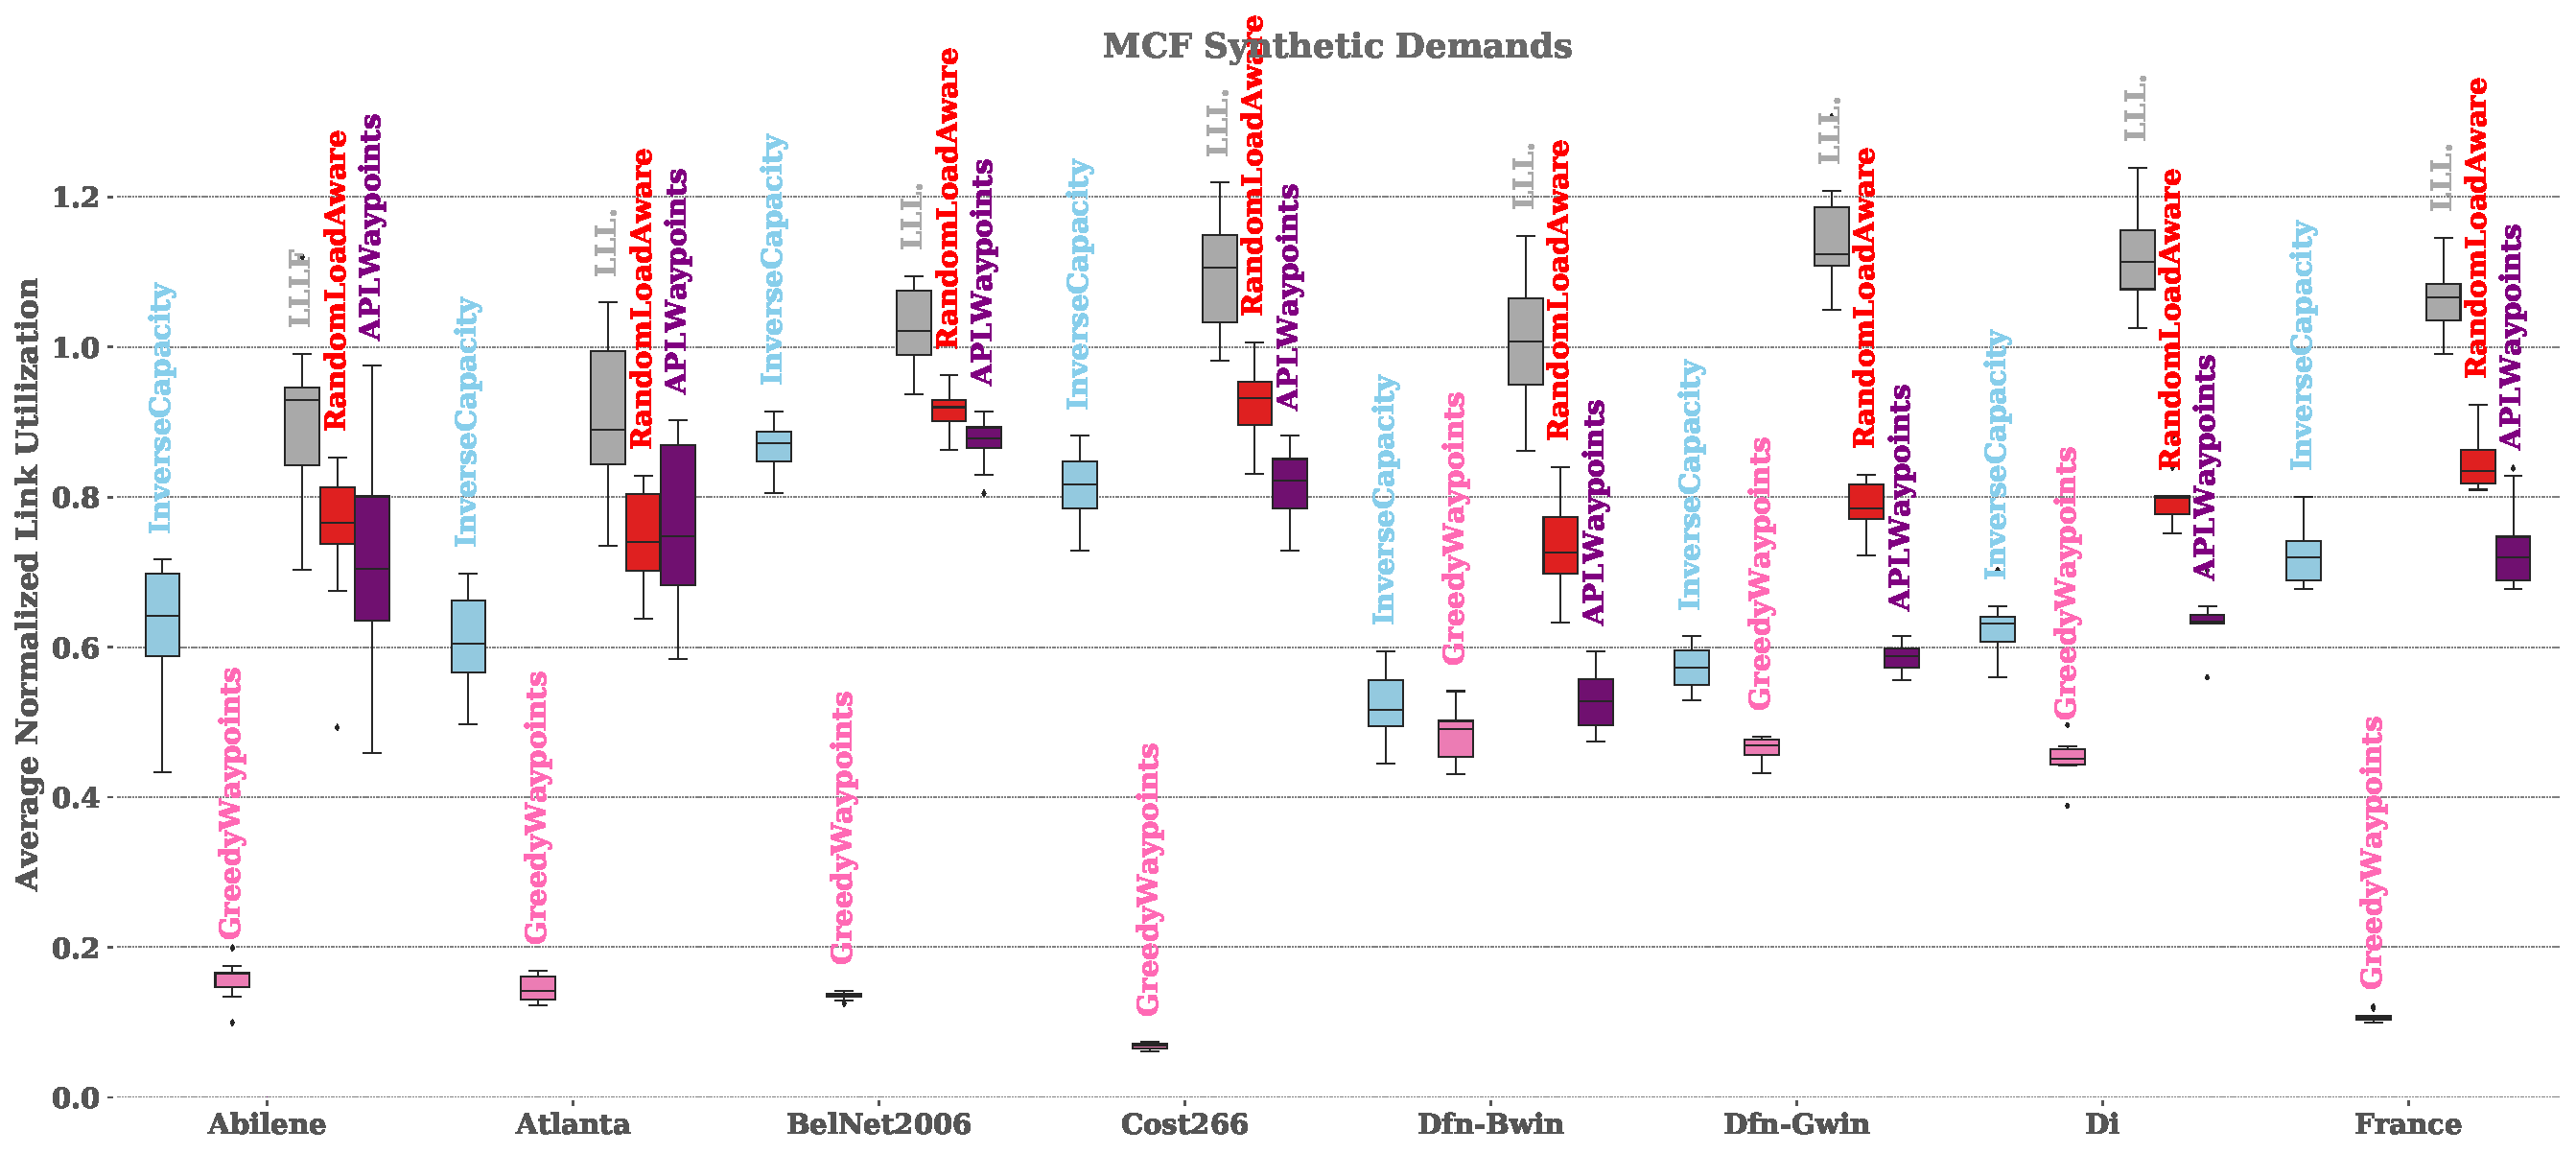
\includegraphics[width=1\linewidth]{Grafiken/projekt1/all_topologies_objective_alu_0.pdf}
               \caption{Synthetische Topologien ALU}
               \label{fig:ergebnisse_projekt_1_synt_topo_alu}
            \end{subfigure}
           \caption{Ergebnisse Projekt 1}
           \label{fig:ergebnisse_projekt_1}
        \end{figure*}
    
        \paragraph{3.2.1   LLLF}
            Die Auswertung der Experimente erfolgte anhand der Metriken Maximal Normalized Link Utilization (MLU) sowie der Ausführungszeit. Die Ergebnisse sind in den Abbildungen aus den Experimenten dargestellt. Man sieht in Abbildung \ref{fig:ergebnisse_projekt_1_synt_topo_mlu}, wie der Algorithmus bei der MLU gut mit den anderen Algorithmen mithalten kann und auch teilweise deutlich besser abschneidet. Diese besonders guten Topologien sind dabei alle sehr dicht, das bedeutet, sie haben viele Kanten und somit auch viele mögliche Pfade. Dadurch hat LLLF eine sehr große Auswahl an möglichen Pfaden und kann die Demands sehr gut auf der Topologie verteilen. 
            Auch sieht man in Abbildung \ref{fig:ergebnisse_projekt_1_synt_topo_time} sehr gut, wie er durchschnittliche genauso schnell läuft, wie die schon vorhandenen Algorithmen.
        
        \paragraph{3.2.2   RLAPS}
            Die Auswertung der Experimente erfolgte anhand der Metriken Average Normalized Link Utilization (ALU), Maximal Normalized Link Utilization (MLU) sowie der Ausführungszeit. Die Ergebnisse sind in den Abbildungen aus den Experimenten dargestellt. Betrachtet man die maximale Linkauslastung (MLU), so wird in Abbildung \ref{fig:ergebnisse_projekt_1_synt_topo_mlu} deutlich, dass RLAPS in nahezu allen getesteten Topologien  eine Verringerung von Hotspots erreicht. Während einfache Verfahren wie Inverse Capacity oder Greedy Waypoints oft hohe Spitzenlasten verursachen, gelingt es RLAPS durch die randomisierte Pfadwahl und lastbasierte Bewertung, die maximale Auslastung einzelner Links abzufedern.
            Ein weiterer Aspekt betrifft die Ausführungszeit, wie in Abbildung \ref{fig:ergebnisse_projekt_1_synt_topo_time} dargestellt. Hier zeigt sich, dass RLAPS zwar deutlich langsamer arbeitet als einfache Verfahren wie Unit Weights, jedoch im Vergleich zu exakten den anderen Ansätzen erheblich schneller ist. Die Implementierung des Algorithmus ist zwar sehr simpel und benötigt lediglich lokale Lastinformationen, die Berechnung von k-kürzesten Pfaden und die wiederholte Bewertung mehrerer Kandidatenpfade führen jedoch zu einem deutlichen Mehraufwand. Besonders auffällig ist, dass die Rechenzeit mit wachsender Topologiegröße und Komplexität exponentiell angestiegen ist, was die praktische Anwendbarkeit in sehr großen Netzwerken einschränken kann. Diese eingeschränkte Skalierbarkeit stellt damit eine der wesentlichen Limitationen von RLAPS dar.
        
        \paragraph{3.2.3   AplWaypoints}
            Zur Bewertung der Leistungsfähigkeit des APL-Waypoint Algorithmus wurden die in der Methodik beschriebenen Metriken Laufzeit, MLU-Auslastung, ALU-Auslastung und APL betrachtet. Im Folgenden werden die Ergebnisse bezüglich jeder der einzelnen Metriken evaluiert. \\
            Bezüglich der Laufzeit zeigt unser Algorithmus eine durchschnittlich sehr geringe Laufzeit über alle Topologien auf. Dabei ist die Laufzeit ungefähr vergleichbar mit den anderen Algorithmen dieser Gruppe und wird lediglich vom InverseCapacity Algorithmus geschlagen, siehe Abbildung \ref{fig:ergebnisse_projekt_1_synt_topo_time}. Die Varianz der Laufzeiten in den Tests bleibt hierbei gering im Allgemeinen und im Vergleich zu den anderen Algorithmen.
            In der Metrik der MLU-Auslastung fällt vor allem die hohe Varianz der MLU-Auslastung auf. Diese zeigt sich unter anderem auch bei Betrachtung der Box-Plots für verschiedene Topologien. Der durchschnittliche Wert der MLU-Auslastung ist vergleichbar schlechter als bei den zum Vergleich gewählten Algorithmen, siehe Abbildung \ref{fig:ergebnisse_projekt_1_synt_topo_mlu}.
            Die Ergebnisse zur Metrik APL, zeigen sehr gute für den APL-Waypoints Algorithmus, siehe \ref{fig:ergebnisse_projekt_1_synt_topo_apl}. Im Allgemeinen schneidet hier unser Algorithmus am besten ab, jedoch nicht deutlich. Des Weiteren haben wir eine tolerierbare Varianz der Ergebnisse, wobei unsere absoluten Minima in fast allen Topologien das beste Ergebnis abbilden.
            Zusammenfassend zeigt APL-Waypoints in allen Metriken vergleichbare Ergebnisse und teilweise gute Ergebnisse. Trotzdem ist hervorzuheben, dass die größte Schwäche in der MLU-Auslastung liegt, welche im Allgemeinen die wichtigste Metrik darstellt. Positiv hervorzuheben ist hierbei vor allem die Laufzeit und die Ergebnisse bezüglich der APL.


\section{Projekt 2}
    Im Anschluss wird das zweite Projekt betrachtet. Ziel war es hierbei, die Algorithmen aus Projekt 1 nicht nur in Simulationen zu untersuchen, sondern sie zusätzlich in einer virtuellen Netzwerkumgebung praktisch anzuwenden.
    
    \subsection{Experimente}
        \paragraph{4.1.1   LLLF}
            \begin{figure*}[h]
                \centering
                \begin{subfigure}[c]{0.34\textwidth}
                    \centering
                    \scalebox{0.75}{
                        \begin{tikzpicture}[
                            node distance=7mm,
                            <->
                            ]
                            \node[state]                    (0)     {$0$};
                            \node[state, above=of 0]        (1)     {$1$};
                            \node[state, above=of 1]        (2)     {$2$};
                            \node[state, above right=of 2]  (3)     {$3$};
                            \node[state, right=of 3]        (4)     {$4$};
                            \node[state, right=of 4]        (5)     {$5$};
                            \node[state, below right=of 5]  (6)     {$6$};
                            \node[state, below=of 6]        (7)     {$7$};
                            \node[state, below=of 7]        (8)     {$8$};
                            \node[state, below left=of 8]   (9)     {$9$};
                            \node[state, left=of 9]         (10)    {$10$};
                    
                            \path (0) edge[left]            node{}       (1);
                            \path (0) edge[bend left, left] node{}       (2);
                            \path (0) edge[left]            node{}       (6);
                            \path (0) edge[left]            node{}       (7);
                            \path (0) edge[left]            node{}       (8);
                            \path (0) edge[left]            node{}       (9);
                            \path (0) edge[left]            node{}       (10);
                            \path (0) edge[left]            node{}       (10);
                            
                            \path (1) edge[left]            node{}       (2);
                            \path (1) edge[left]            node{}       (3);
                            \path (1) edge[left]            node{}       (4);
                            \path (1) edge[left]            node{}       (5);
                            \path (1) edge[left]            node{}       (7);
                            \path (1) edge[left]            node{}       (9);
                            \path (1) edge[left]            node{}       (10);
                            
                            \path (2) edge[left]            node{}       (4);
                            \path (2) edge[left]            node{}       (5);
                            \path (2) edge[left]            node{}       (7);
                            \path (2) edge[left]            node{}       (8);
                            \path (2) edge[left]            node{}       (9);
                            \path (2) edge[left]            node{}       (10);
                            
                            \path (3) edge[left]            node{}       (4);
                            \path (3) edge[bend left, left] node{}       (5);
                            \path (3) edge[left]            node{}       (6);
                            \path (3) edge[left]            node{}       (7);
                            \path (3) edge[left]            node{}       (8);
                            \path (3) edge[left]            node{}       (9);
                            \path (3) edge[left]            node{}       (10);
                            
                            \path (4) edge[left]            node{}       (5);
                            \path (4) edge[left]            node{}       (6);
                            \path (4) edge[left]            node{}       (7);
                            \path (4) edge[left]            node{}       (8);
                            
                            \path (5) edge[left]            node{}       (7);
                            \path (5) edge[left]            node{}       (9);
                            \path (5) edge[left]            node{}       (10);
                            
                            \path (6) edge[left]            node{}       (7);
                            \path (6) edge[bend left, left] node{}       (8);
                            \path (6) edge[left]            node{}       (9);
                            \path (6) edge[left]            node{}       (10);
                            
                            \path (7) edge[left]            node{}       (9);
                            \path (7) edge[left]            node{}       (10);
                            
                            \path (8) edge[left]            node{}       (9);
                            \path (8) edge[left]            node{}       (10);
                        \end{tikzpicture}
                    }
                    \caption{LLLF-Topologie}
                    \label{fig:ergebnisse_projekt_2_lllf_topologie} 
                \end{subfigure}
                \begin{subfigure}[c]{0.64\textwidth}
                    \centering
                    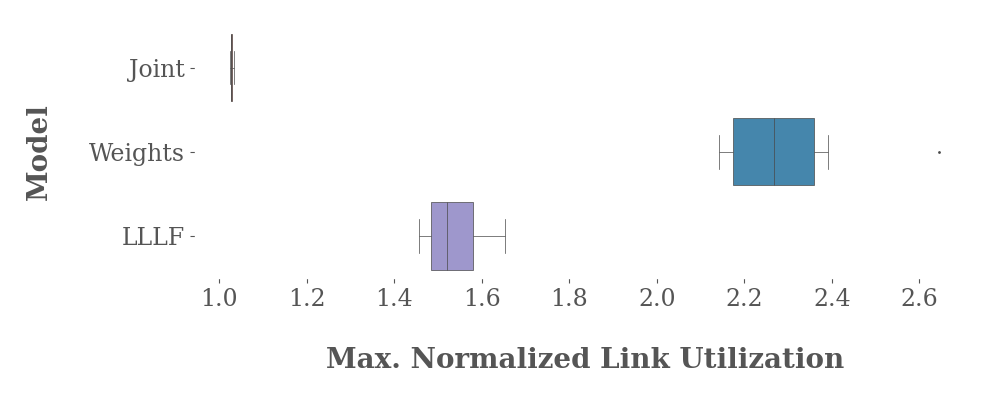
\includegraphics[width=\textwidth]{Grafiken/projekt2/result_lllf.png}
                    \caption{Ergebnisse LLLF Projekt 2}
                    \label{fig:ergebnisse_projekt_2_lllf_ergebnisse}
                \end{subfigure}
                \caption{Ergebnisse LLLF Projekt 2}
                \label{fig:ergebnisse_projekt_2_lllf}
            \end{figure*}
            Um im zweiten Projekt gute Ergebnisse mit LLLF zu erzielen, haben eine neue sehr dichte Topologie \ref{fig:ergebnisse_projekt_2_lllf_topologie} entworfen, auf welcher LLLF sehr gut klarkommen sollte. Dabei haben alle Kanten eine Kapazität von $2$ und alle Demands sind $1$ groß. Die theoretisch mögliche MLU ist $0,5$.
        
        \paragraph{4.1.2   RLAPS}
            Im zweiten Experiment wurde die Topologie aus Abbildung \ref{fig:ergebnisse_projekt_2_rlaps_topologie} entworfen, die gezielt gut geeignet für Randomized Load-Aware Path Selection (RLAPS) ist. Sie bietet eine hohe Pfadvielfalt, wodurch die randomisierte Vorauswahl tatsächlich verschiedene Alternativen berücksichtigen kann. Zentrale Engpässe wurden vermieden, sodass Lasten besser verteilt werden können. Die Kapazitäten wurden konsistent modelliert, um die Bewertungsfunktion nicht zu verzerren und die Netzgröße wurde moderat gehalten, damit die Berechnung der $k$-kürzesten Pfade handhabbar bleibt für die Testumgebung. Zusätzlich wurden für die Reproduzierbarkeit der Ergebnisse Anpassungen an den Bitraten vorgenommen, sodass die Experimente zügig wiederholt werden können.
            \begin{figure*}[h]
                \centering
                \begin{subfigure}[c]{0.34\textwidth}
                    \centering
                    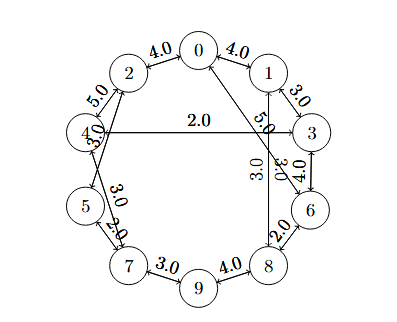
\includegraphics[width=1\linewidth]{Grafiken/projekt2/Topologie RLAPS.png}
                    \caption{RLAPS-Topologie}
                    \label{fig:ergebnisse_projekt_2_rlaps_topologie}
                \end{subfigure}
                \begin{subfigure}[c]{0.64\textwidth}
                    \centering
                    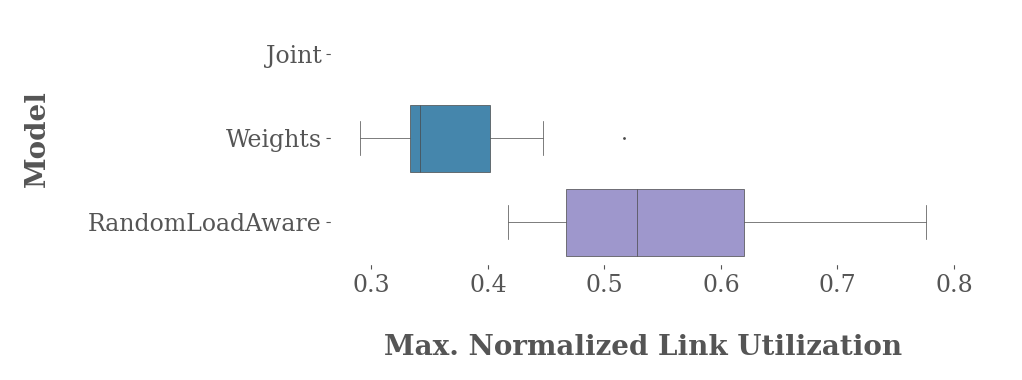
\includegraphics[width=1\linewidth]{Grafiken/projekt2/results_compare_rla.png}
                    \caption{Ergebnisse RLAPS Projekt 2}
                    \label{fig:ergebnisse_projekt_2_rlaps_ergebnisse}
                \end{subfigure}
                \caption{Ergebnisse RLAPS Projekt 2}
                \label{fig:ergebnisse_projekt_2_rlaps}
            \end{figure*}
            
        \paragraph{4.1.3   AplWaypoints}
            Für einen realitätsnahen Vergleich werden in Experiment 2 die Algorithmen JOINT, Weights und APL-Waypoints in dem Simulationsframework nanonet betrachtet. Dabei hat jeder Algorithmus eine individuell definierte Topologie sowie eine eigen definiertes Routingverhalten.
            
            Dabei wurde für den APL-Waypoints Algorithmus eine Grid-Topologie ausgewählt, siehe Abbildung \ref{fig:ergebnisse_projekt_2_apl_waypoints_topologie}. Dieses bietet unserem Algorithmus neben der hohen Pfaddiversität eine Kapazitätssetzung, die Umwege um den zentralen Pfad einen erhöhten Mehrwert geben. Des Weiteren wurde neben der Bitrate die Topologie klein gehalten in der Definition der nötigen Dateien, um die Durchlaufzeit gering zu halten.

            \begin{figure*}[h]
                \centering
                 \begin{subfigure}[c]{0.34\textwidth}
                    \centering
                    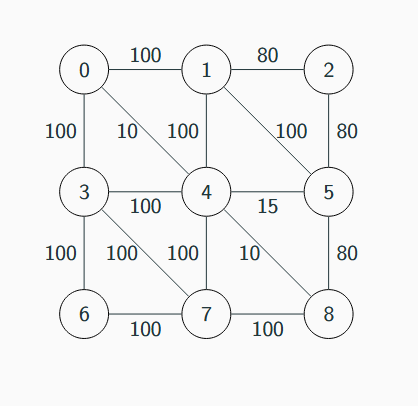
\includegraphics[width=0.9\linewidth]{Grafiken/projekt2/apl_waypoints_grid_topo.png}
                    \caption{APL-Waypoints-Topologie}
                    \label{fig:ergebnisse_projekt_2_apl_waypoints_topologie}
                \end{subfigure}
                \begin{subfigure}[c]{0.64\textwidth}
                    \centering
                    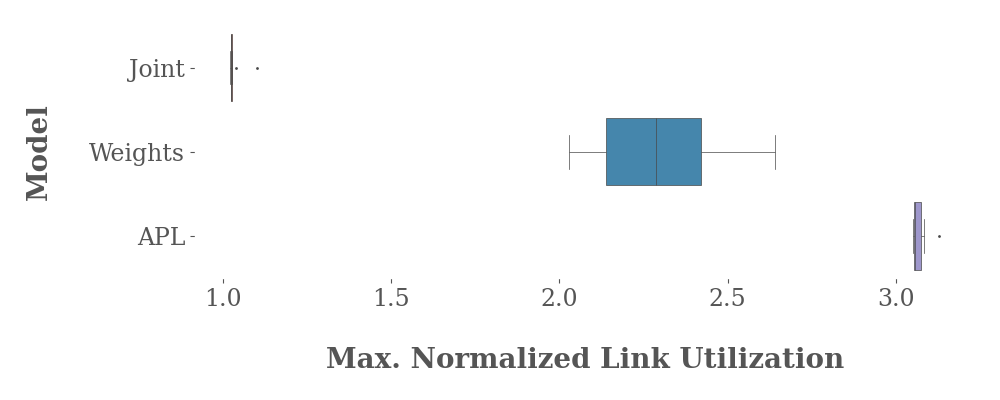
\includegraphics[width=1\linewidth]{Grafiken/projekt2/result_apl_1.png}
                    \caption{Ergebnisse APL-Waypoints Projekt 2}
                    \label{fig:ergebnisse_projekt_2_apl_waypoints_ergebnisse}
                \end{subfigure}
                \caption{Ergebnisse APL Projekt 2}
                \label{fig:ergebnisse_projekt_2_apl_waypoints}
            \end{figure*}
            
    \subsection{Resultate}
        \paragraph{4.2.1   LLLF}
            In Abbildung \ref{fig:ergebnisse_projekt_2_lllf_ergebnisse} kann man sehen wie, der Weights-, der Joint- und der LLLF-Algorithmus abgeschnitten haben. Man sieht, dass LLLF zwischen Joint und Weights liegt. Es fällt aber auch auf, dass die eigentliche theoretische MLU von $0,5$ nicht erreicht wurde. Das könnte an einigen Fehlern bei der Simulation liegen, die während der ersten paar Minuten häufiger aufgetreten sind, dann aber verschwanden.
        
        \paragraph{4.2.2   RLAPS}
            RLAPS wurde direkt mit der Weights-Methode auf der erstellten Topologie verglichen (vgl. Abbildung \ref{fig:ergebnisse_projekt_2_rlaps_ergebnisse}). Während Weights eine konsistent niedrigere maximale Linkauslastung erzielt und nur geringe Varianz aufweist, zeigt RLAPS ein deutlich breiteres Ergebnisintervall. Der Median der MLU liegt bei RLAPS höher, was auf tendenziell schlechtere Ergebnisse hindeutet. Gleichzeitig belegen die Ausreißer nach unten, dass RLAPS in einzelnen Durchläufen durchaus konkurrenzfähige Resultate liefern kann.
            Die Randomisierung schafft Diversität in der Pfadwahl und kann Hotspots wirksam vermeiden, führt aber auch zu höherer Ergebnisvarianz. Während deterministische Verfahren wie Weights eine stabile, aber weniger flexible Lösung bieten, bewegt sich RLAPS zwischen sehr guten und weniger guten Resultaten. Für praktische Anwendungen bedeutet dies, dass RLAPS eher als explorativer Ansatz geeignet ist, dessen Leistungsfähigkeit durch mehrere Läufe und Mittelwertbildung abgesichert werden sollte.
        
        
        \paragraph{4.2.3   AplWaypoints}
            Der APL-Waypoints Algorithmus zeigt auch im Experiment 2 vergleichbare Ergebnisse. Dabei zeigt Abbildung \ref{fig:ergebnisse_projekt_2_apl_waypoints_ergebnisse} die MLU in Bezug auf die gegebenen Demands.  APL-Waypoints zeigt hier eine deutlich höhere MLU, siehe Abbildung \ref{fig:ergebnisse_projekt_2_apl_waypoints_ergebnisse}, im Vergleich zu JOINT und Weights. Jedoch zeigt hier unser Algorithmus ein sehr stabiles Ergebnis, gekennzeichnet durch die ausgesprochen niedrige Varianz. Dies unter der hohen Belastung zeigt die Robustheit des Algorithmus. 
            Im Allgemeinen hebt Experiment 2 die schon in Experiment 1 erkannte Schwäche des APL-Waypoint Algorithmus erneut hervor. Die Werte in der Metrik der MLU zeigen einen generellen Nachteil gegenüber den zum Vergleich herangezogenen Algorithmen. Dabei ist positiv lediglich die geringe Varianz und somit die hohe Stabilität der Ergebnisse hervorzuheben. Zusammenfassend schneidet APL-Waypoints, in Bezug auf lediglich die Ergebnisse von Experiment 2, vergleichsweise schlecht ab.

\section{Reproduktion}
    Die Reproduktion der Projekte aus Gruppe 4 verlief insgesamt erfolgreich. Wesentliche
    Abweichungen von den ursprünglichen Ergebnissen konnten wir nicht feststellen.
    Bei Projekt 1 war der Code gut dokumentiert und strukturiert. Die Ausführung sowie die grafischen Darstellungen funktionierten ohne Probleme, und die Resultate entsprachen den Originalen.
    Auch Projekt 2 ließ sich problemlos ausführen. Auffällig war lediglich, dass unsere Ergebnisse etwas besser ausfielen, was vermutlich auf Unterschiede in der Testumgebung zurückzuführen ist. Insgesamt bestätigten unsere Experimente die ursprünglichen Resultate. Die Leistung unserer Algorithmen ordnete sich konsistent in die bestehenden Verfahren ein.

\section{Zusammenfassung}
    Im Gesamten lief die Einarbeitung unserer Algorithmen gut. Es gab zwar an einigen Stellen Schwierigkeiten, sich in die Projekte einzuarbeiten und unsere Algorithmen passend zu implementieren. Auch hat die Analyse von APL und ALU in den schon implementierten Algorithmen zu weiterem Aufwand geführt, aber diese Schwierigkeiten konnten überwunden werden. Die Ergebnisse der Algorithmen waren dabei gemischt. Teilweise waren sie schneller als die schon existierenden Algorithmen, teilweise aber auch langsamer. Unsere Algorithmen haben sich dabei also gut in die schon existierenden aufgereiht. \\


%%
%% The next two lines define the bibliography style to be used, and
%% the bibliography file.
\bibliographystyle{ACM-Reference-Format}
\bibliography{sample-base}


% %%
% %% If your work has an appendix, this is the place to put it.
% \appendix

% \section{Research Methods}

% \subsection{Part One}

% Lorem ipsum dolor sit amet, consectetur adipiscing elit. Morbi
% malesuada, quam in pulvinar varius, metus nunc fermentum urna, id
% sollicitudin purus odio sit amet enim. Aliquam ullamcorper eu ipsum
% vel mollis. Curabitur quis dictum nisl. Phasellus vel semper risus, et
% lacinia dolor. Integer ultricies commodo sem nec semper.

% \subsection{Part Two}

% Etiam commodo feugiat nisl pulvinar pellentesque. Etiam auctor sodales
% ligula, non varius nibh pulvinar semper. Suspendisse nec lectus non
% ipsum convallis congue hendrerit vitae sapien. Donec at laoreet
% eros. Vivamus non purus placerat, scelerisque diam eu, cursus
% ante. Etiam aliquam tortor auctor efficitur mattis.

% \section{Online Resources}

% Nam id fermentum dui. Suspendisse sagittis tortor a nulla mollis, in
% pulvinar ex pretium. Sed interdum orci quis metus euismod, et sagittis
% enim maximus. Vestibulum gravida massa ut felis suscipit
% congue. Quisque mattis elit a risus ultrices commodo venenatis eget
% dui. Etiam sagittis eleifend elementum.

% Nam interdum magna at lectus dignissim, ac dignissim lorem
% rhoncus. Maecenas eu arcu ac neque placerat aliquam. Nunc pulvinar
% massa et mattis lacinia.

\end{document}
\endinput
%%
%% End of file `sample-sigconf.tex'.
